% main.tex — Project Simurgh IEEE Conference Paper
\documentclass[conference]{IEEEtran}
\usepackage[utf8]{inputenc}
\usepackage[T1]{fontenc}
\usepackage{graphicx}
\usepackage{xcolor}
\usepackage{listings}
\usepackage{tikz}
\usepackage{amsmath,amssymb}
\usepackage{cite}
\usepackage{booktabs}
\usepackage{tabularx}
\usepackage{url}
\usepackage{microtype}
\usepackage{orcidlink}
\usepackage{hyperref}
\hypersetup{
  pdftitle={Project Simurgh: Privacy-Preserving Device Integrity Proofs for Capture-Resistant High-Stakes Sessions},
  pdfauthor={Mohammad Raouf Abedini},
  pdfkeywords={academic integrity, device attestation, display affinity, Ed25519, ECDSA P-256, integrity proofs, online proctoring, privacy-preserving, WebRTC},
  colorlinks=true,
  linkcolor=black,
  citecolor=black,
  urlcolor=blue
}
\def\UrlBreaks{\do\/\do-\do_\do.\do=\do?\do&\do\#}
\usetikzlibrary{shapes,arrows.meta,positioning,fit,backgrounds,calc}

\lstset{
  basicstyle=\ttfamily\footnotesize,
  breaklines=true,
  frame=single,
  numbers=left,
  numberstyle=\tiny\color{gray},
  keywordstyle=\color{blue},
  commentstyle=\color{green!50!black},
  stringstyle=\color{red},
  columns=fullflexible
}

\IEEEoverridecommandlockouts

\begin{document}

\title{Project Simurgh: Privacy-Preserving Device Integrity Proofs for Capture-Resistant High-Stakes Sessions}

\author{\IEEEauthorblockN{Mohammad Raouf Abedini\,\orcidlink{0009-0000-6214-258X}}
\IEEEauthorblockA{Department of Computing\\
Macquarie University\\
Sydney, Australia\\
mohammadraouf.abedini@students.mq.edu.au\\
\url{https://raoufabedini.dev}}
\thanks{LLM-assisted development methodology disclosed in Section~VIII-F.}}

\maketitle

%% ===================================================================
%% ABSTRACT
%% ===================================================================
\begin{abstract}
Project Simurgh is a privacy-preserving integrity architecture for high-stakes AI-mediated and remote assessment sessions. Existing browser-based proctoring systems commonly treat screen-capture output as a faithful representation of the physical display. However, documented operating-system display-affinity behaviours on Windows and macOS show that visible windows can be omitted from capture surfaces, invalidating capture-based trust assumptions~\cite{abedini2026invisible}.

Simurgh responds by replacing surveillance-first visual monitoring with signed, metadata-only integrity proofs. The system combines browser behavioural telemetry, local device integrity daemons, cryptographic challenge-response proofs (Ed25519 for the browser-paired integrity-proof envelope; ECDSA P-256 for the cross-platform device-shield daemons), native OS metadata scanners, server-side verification, and HMAC-SHA256-linked tamper-evident audit trails. It does not collect screen pixels, webcam frames, microphone audio, typed content, pasted content, raw process names, raw window titles, window handles, process identifiers, or personal device identifiers. Every anomaly is treated as a signal for human review; no automatic misconduct finding is ever produced.

We implement Simurgh as a cross-platform research prototype spanning a Node.js verifier, a browser SDK, and localhost daemons for macOS (Swift/CryptoKit), Windows (.NET), and Linux (Rust). The Windows Device Shield validates detection of \texttt{WDA\_MONITOR} and \texttt{WDA\_EXCLUDEFROMCAPTURE} on Windows~10 Pro build~19045. The Linux research path adds signed daemon proofs, X11 window-state metadata coverage, Wayland portal property probing, XWayland partial coverage, display-server mismatch enforcement, and development systemd user lifecycle support. Automated validation includes 327 Node.js unit tests, 33 Rust tests, 11 Windows .NET tests, 8 macOS Swift tests, end-to-end smoke tests, cybersecurity audits, privacy audits, and CI gates.

This paper presents Simurgh's threat model, architecture, proof protocol, privacy contract, platform implementations, evaluation results, limitations, and ethical deployment boundaries. We argue that capture-resistant integrity systems should verify signed environment metadata rather than collect more invasive surveillance data.
\end{abstract}

\begin{IEEEkeywords}
academic integrity, device attestation, display affinity, Ed25519, ECDSA P-256, integrity proofs, online proctoring, privacy-preserving security, screen capture evasion
\end{IEEEkeywords}

%% ===================================================================
%% SECTION I: INTRODUCTION
%% ===================================================================
\section{Introduction}

Remote proctoring systems that monitor examinations through the WebRTC \texttt{getDisplayMedia()} API~\cite{bruaroey2025screen} rest on a single implicit assumption: the captured frame faithfully represents the physical display. Prior work has shown this assumption is false~\cite{abedini2026invisible}. Both Windows and macOS expose documented, user-level OS APIs that exclude application windows from all screen-capture pipelines while leaving them fully visible on the physical monitor. Commercial AI-overlay tools already exploit these APIs to provide live AI assistance during examinations and technical interviews, invisible to any capture-based monitoring system~\cite{cluely2025,interviewcoder2026,fabrichq2026cheating}.

The defensive response cannot simply be ``capture more.'' Existing proctoring approaches already collect webcam feeds, gaze streams, keystroke content, audio, and full-screen video, imposing well-documented psychological costs~\cite{conijn2022fear} and raising serious privacy concerns~\cite{paris2021sins,mukherjee2024balancing}. Adding hardware capture cards or GPU-level frame hooks compounds the privacy problem while still being defeatable by sufficiently motivated adversaries.

\textit{Project Simurgh} takes a different path. Rather than attempting to close the gap between the physical display and the capture surface, Simurgh abandons that surface entirely as a trust anchor. Instead, it establishes session integrity through signed, metadata-only device proofs: the local integrity daemon attests to its own identity and environment state using ECDSA P-256 over SHA-256~\cite{fips1865}, while the browser-paired integrity-proof envelope uses Ed25519~\cite{rfc8032}; the server verifies each proof against the session's registered key; and every accept and reject event is written to an HMAC-SHA256-linked audit chain~\cite{rfc2104} that any inspector can verify offline. No screen pixels, webcam frames, audio, typed content, pasted content, raw process names, raw window titles, or personal device identifiers are collected at any layer.

This paper makes the following contributions:

\begin{itemize}
\item \textbf{Privacy-preserving integrity architecture}: We design and implement a system that replaces visual surveillance with signed metadata-only proofs, demonstrating that session integrity can be assessed without collecting any content-level data.

\item \textbf{Cross-platform research prototype}: We implement Simurgh as a working system spanning a browser telemetry SDK, a Node.js verifier, and localhost integrity daemons for macOS (Swift/CryptoKit), Windows (.NET), and Linux (Rust), unified under a common proof contract.

\item \textbf{OS-level display-affinity detection without screen capture}: We show that the display-affinity risk class documented in~\cite{abedini2026invisible} can be detected through native OS metadata scanners that report window-count summaries without ever accessing window content, titles, or identifiers.

\item \textbf{Evaluated prototype with manual-review-only decision model}: We evaluate the system through 379 automated tests across four language runtimes (Node.js, Rust, .NET, and Swift), end-to-end smoke tests, cybersecurity and privacy audits, and real-device Windows validation, while preserving the invariant that every anomaly signal requires a human reviewer to reach any integrity conclusion.
\end{itemize}

The remainder of this paper is organised as follows. Section~II motivates the capture-fidelity failure and privacy problems with existing proctoring. Section~III presents the threat model and design goals. Section~IV describes the system architecture. Section~V details the proof protocol. Section~VI covers platform implementations. Section~VII specifies the privacy model. Section~VIII reports the evaluation. Section~IX analyses security properties and remaining attacks. Section~X addresses ethics and deployment limits. Section~XI surveys related work. Section~XII discusses future directions. Section~XIII concludes.

%% ===================================================================
%% SECTION II: MOTIVATION
%% ===================================================================
\section{Motivation: The Capture-Fidelity Failure}

\subsection{The Invisible Window Attack}

The motivating vulnerability for this work is the Invisible Window attack class, formally documented in~\cite{abedini2026invisible}. Both Windows 10~v2004+ and macOS provide documented, user-level APIs that exclude application windows from all screen-capture pipelines while maintaining their visibility on the physical display. On Windows, \texttt{SetWindowDisplayAffinity} with the \texttt{WDA\_EXCLUDEFROMCAPTURE} flag~\cite{microsoft2025setwindow} causes a window to produce no pixels in any capture output. On macOS, \texttt{NSWindow.SharingType.none}~\cite{apple2025sharingtype} achieves an equivalent effect through the CoreGraphics capture pipeline. Both Apple Product Security and Microsoft MSRC classified these behaviours as consistent with documented functionality and by-design, respectively~\cite{abedini2026invisible}. Empirical evaluation in~\cite{abedini2026invisible} confirmed 100\% evasion across Windows~10/11, macOS~14, and macOS~26.3.1, with zero visual artefacts.

Three distinct subclasses exist: (1)~capture-invisible overlays using \texttt{WDA\_EXCLUDEFROMCAPTURE} or \texttt{SharingType.none}, undetectable from any DOM event or \texttt{getDisplayMedia()} stream; (2)~click-through overlays using \texttt{WS\_EX\_TRANSPARENT} or \texttt{ignoresMouseEvents}, which do not fire focus/blur events in the exam browser; and (3)~GPU-layer overlays that hook DirectX or Metal directly, bypassing both DOM events and the OS capture pipeline. Commercial tools such as Cluely~\cite{cluely2025} and Interview Coder~\cite{interviewcoder2026} combine these techniques, and a 2026 industry survey estimated that 35\% of candidates in technical assessments showed signs of AI-assisted cheating~\cite{fabrichq2026cheating}.

\subsection{Why Screen Capture Is the Wrong Trust Boundary}

The WebRTC Screen Capture API~\cite{bruaroey2025screen} delegates pixel composition entirely to the OS compositing pipeline. The browser has no mechanism to detect omissions from that pipeline; it receives a valid-looking frame that simply does not include excluded windows. As~\cite{abedini2026invisible} formalises:

\begin{quote}
\textbf{Display Fidelity Property.} A capture system satisfies display fidelity if and only if the captured frame $F$ is pixel-identical to the physical display output $D$ for all visible screen regions.
\end{quote}

This property does not hold on any tested platform when any visible window has a capture-exclusion flag set. The trust boundary proctoring systems implicitly rely on --- that the OS faithfully reports what the user sees --- is structurally absent from the current platform landscape. Adding more resolution, frame rate, or webcam channels does not address the structural gap; it increases the surveillance cost without closing the attack surface.

\subsection{Privacy Problems with Surveillance-First Proctoring}

Current proctoring platforms collect webcam video, microphone audio, gaze streams, keystrokes, screen recordings, browser histories, and system process lists~\cite{balash2023educators,balash2021examining}. Research consistently documents the privacy, equity, and psychological harms of this model: elevated student anxiety~\cite{conijn2022fear}, algorithmic bias in facial recognition~\cite{mukherjee2024balancing}, and structural privacy violations in e-learning systems~\cite{paris2021sins}. Vulnerability in student digital well-being under AI-powered educational decision systems is a specific emerging concern~\cite{prinsloo2024vulnerable}. Even setting aside the attack surface, the surveillance model imposes costs that may not be justified by its integrity benefits~\cite{duncan2022necessity,khalil2022nexus}.

Simurgh's design premise is that these costs are unnecessary. Session integrity can be assessed through metadata that does not include any user-generated content, and anomaly signals can be surfaced for human review without ever building a pixel-level record of the student's screen.

%% ===================================================================
%% SECTION III: THREAT MODEL AND DESIGN GOALS
%% ===================================================================
\section{Threat Model and Design Goals}

\subsection{Adversary Model}

The adversary is a test-taker with standard (non-administrator) access to their own computer who wishes to consult unauthorised AI assistance during an assessment. The adversary can run compiled native applications, control all software on their machine, and install browser extensions. The adversary cannot modify the proctoring server, the exam platform, or the OS kernel. The adversary is specifically capable of deploying capture-invisible overlays of all three subclasses described in Section~II-A.

\subsection{Attacker Capabilities Against Capture-Based Systems}

Against a browser-only proctoring system that relies solely on \texttt{getDisplayMedia()}, the adversary can achieve complete evasion by deploying a \texttt{WDA\_EXCLUDEFROMCAPTURE}-flagged or \texttt{SharingType.none} window. No DOM event, no \texttt{getDisplayMedia()} artefact, and no browser-observable state change reveals the presence of the overlay. This is the baseline attack that motivates the Simurgh architecture.

\subsection{What Native OS Metadata Can Provide}

Unlike the browser capture pipeline, the OS window-management layer retains records of all top-level windows regardless of their capture-exclusion state. On Windows, \texttt{GetWindowDisplayAffinity} returns the affinity flag for any enumerable window. On macOS, \texttt{CGWindowListCopyWindowInfo} returns the \texttt{kCGWindowSharingState} property for all windows. These metadata APIs are accessible to any native process with standard user privileges. Crucially, they report exclusion \textit{presence} without reading window content, titles, or process names. Simurgh's native daemons exploit this gap: they run at the OS level where the capture-exclusion flag is visible, sign a summary of the metadata, and transmit the signed proof to the verifier.

\subsection{Design Goals}

\begin{enumerate}
\item \textbf{Capture independence}: Session integrity must be assessable without any screen, webcam, audio, or content capture.

\item \textbf{Privacy preservation}: No typed content, pasted content, raw window titles, raw process names, window handles, process identifiers, or personal device identifiers may be collected at any layer.

\item \textbf{Cryptographic verifiability}: Every accepted or rejected integrity signal must be signed by the device daemon and written to a tamper-evident server-side audit chain, making post-hoc modification detectable in exported audit records.

\item \textbf{Replay resistance}: A captured proof from session $S$ must not be replayable in session $S'$.

\item \textbf{Manual-review-only decision model}: No component of the system may produce an automatic misconduct finding. Every anomaly signal is an input to a human reviewer.

\item \textbf{Honest non-claims}: The system must not claim capabilities it does not have. GPU-layer overlays, kernel-level compromises, read-only workflows, and hardware-rooted attestation are explicitly out of scope.
\end{enumerate}

%% ===================================================================
%% SECTION IV: SYSTEM OVERVIEW
%% ===================================================================
\section{System Overview}

Figure~\ref{fig:architecture} shows the high-level system architecture. Simurgh operates as four coordinated layers: a browser telemetry SDK, a local integrity daemon, a Node.js verifier/server, and an instructor reporting and audit layer.

%% ─── Figure 1: System Architecture ───
\begin{figure*}[t]
\centering
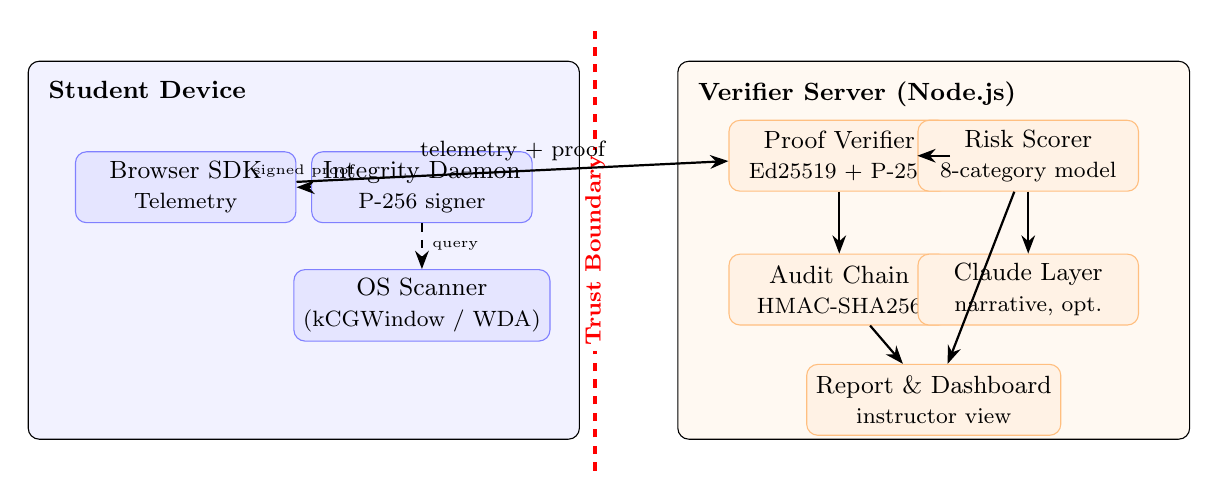
\begin{tikzpicture}[
  >=Stealth,
  box/.style={draw, rounded corners, minimum width=2.8cm, minimum height=0.9cm, align=center, font=\small},
  bigbox/.style={draw, rounded corners, align=center},
  arr/.style={->, thick},
]

% Student device
\node[bigbox, fill=blue!5, minimum width=7cm, minimum height=4.8cm] (device) at (0,0) {};
\node[font=\small\bfseries, anchor=north west] at ([xshift=4pt,yshift=-4pt] device.north west) {Student Device};

\node[box, fill=blue!10, draw=blue!50] (sdk)    at (-1.5, 0.8) {Browser SDK\\{\footnotesize Telemetry}};
\node[box, fill=blue!10, draw=blue!50] (daemon) at ( 1.5, 0.8) {Integrity Daemon\\{\footnotesize P-256 signer}};
\node[box, fill=blue!10, draw=blue!50] (scanner) at (1.5, -0.7) {OS Scanner\\{\footnotesize (kCGWindow / WDA)}};

\draw[arr, dashed] (daemon) -- (scanner) node[right, font=\tiny, midway] {query};
\draw[arr] (daemon) -- node[above, font=\tiny] {signed proof} (sdk);

% Trust boundary
\draw[red, dashed, line width=1.5pt] (3.7, -2.8) -- (3.7, 2.8);
\node[font=\footnotesize\bfseries, red, fill=white, inner sep=2pt, rotate=90] at (3.7, 0) {Trust Boundary};

% Server side
\node[bigbox, fill=orange!5, minimum width=6.5cm, minimum height=4.8cm] (server) at (8.0, 0) {};
\node[font=\small\bfseries, anchor=north west] at ([xshift=4pt,yshift=-4pt] server.north west) {Verifier Server (Node.js)};

\node[box, fill=orange!10, draw=orange!50] (verifier)  at (6.8, 1.2) {Proof Verifier\\{\footnotesize Ed25519 + P-256}};
\node[box, fill=orange!10, draw=orange!50] (risk)      at (9.2, 1.2) {Risk Scorer\\{\footnotesize 8-category model}};
\node[box, fill=orange!10, draw=orange!50] (audit)     at (6.8,-0.5) {Audit Chain\\{\footnotesize HMAC-SHA256}};
\node[box, fill=orange!10, draw=orange!50] (claude)    at (9.2,-0.5) {Claude Layer\\{\footnotesize narrative, opt.}};
\node[box, fill=orange!10, draw=orange!50] (report)    at (8.0,-1.9) {Report \& Dashboard\\{\footnotesize instructor view}};

\draw[arr] (verifier) -- (risk);
\draw[arr] (verifier) -- (audit);
\draw[arr] (risk) -- (claude);
\draw[arr] (risk) -- (report);
\draw[arr] (audit) -- (report);

% Cross-boundary arrows
\draw[arr, thick] (sdk) -- node[above, font=\footnotesize] {telemetry + proof} (verifier);

\end{tikzpicture}
\caption{Simurgh system architecture. The student device runs a browser SDK (telemetry collection) and a local integrity daemon (ECDSA P-256-signed proofs of OS metadata; the browser-paired integrity-proof envelope uses Ed25519). The daemon queries OS-level window-state metadata without accessing content. All proof material crosses the trust boundary to the Node.js verifier, which checks signatures, scores risk, appends to the audit chain, optionally invokes the Claude narrative layer, and exposes a read-only instructor dashboard and report.}
\label{fig:architecture}
\end{figure*}

\subsection{Browser Telemetry Layer}

The browser SDK, embedded in the exam page, collects a behavioural metadata stream covering approximately 18 browser-side behavioural event types; the full event registry (\texttt{src/academic/academicEvents.js}) additionally defines pairing, daemon-proof, scanner, and session-lifecycle events emitted server-side. The collected signals include: keystroke count (not content), character-typed count (not content), paste event count and character length (not paste content), focus-loss count and duration, idle-gap maxima, effective words-per-minute rate, and keydown timing intervals (up to 200 samples, no content). The raw student identifier is hashed with SHA-256 at server ingress; the raw value is never written to disk, logged, or transmitted further.

The telemetry stream is deliberately narrow. No DOM content, no clipboard text, no window titles, no \texttt{getDisplayMedia()} stream, and no webcam feed are collected.

\subsection{Local Integrity Daemon}

The integrity daemon is a native process running on the student's machine at \texttt{127.0.0.1}. Its responsibilities are:
\begin{enumerate}
\item Maintain an ECDSA P-256 key pair: persistent on macOS (stored in the macOS Keychain under account \texttt{p256-signing-key}) and on Linux (an identity file at mode \texttt{0600} within a \texttt{0700} state directory under \texttt{\$XDG\_STATE\_HOME}); the current Windows research daemon generates the key ephemerally for the lifetime of the process, with persistent storage backed by DPAPI deferred to a future stage.
\item On request, query OS metadata APIs to obtain the current display-affinity window summary.
\item Construct a signed proof envelope containing the version, platform, session identifier, node identity hash, timestamp, nonce, \texttt{capabilities} sub-object (four boolean scanner-capability flags), \texttt{signals} sub-object (window counts and helper status), privacy mode, and ECDSA P-256 signature over the canonical serialisation of all non-signature fields.
\item Respond to pairing challenges issued by the server.
\end{enumerate}

The daemon explicitly does not enumerate window titles, process names, process identifiers, raw window handles, or any content-level data. The OS scanner returns a count of windows with capture-exclusion flags set, not a list of which windows or what they display.

\subsection{Server Verifier}

The Node.js server receives telemetry events and proof envelopes from the browser SDK. For each proof, it performs the following verification steps, detailed further in Section~V:
\begin{enumerate}
\item Schema validation: all eleven required fields must be present and correctly typed.
\item Nonce check: the nonce must not have been seen in this session (replay guard).
\item Signature verification: Ed25519 \texttt{verify(canonical, pubkey, sig)} for the browser-paired proof envelope; ECDSA P-256 over SHA-256 for the device-shield daemon envelope.
\item Node continuity: the submitting node's hash must match the bound node for this session.
\item Audit append: the result (accept or reject with reason) is written to the HMAC chain.
\end{enumerate}

Risk scoring aggregates telemetry events and proof results into a session risk score across eight weighted categories: paste behaviour, focus events, typing patterns, idle periods, display-affinity signals, helper connection state, daemon proof signals, and session lifecycle. The risk scorer produces three fixed verdict strings, hard-coded and unsuppressable through configuration:
\begin{itemize}
\item \textbf{Critical}: ``Manual review required. No automatic misconduct finding.''
\item \textbf{Warning}: ``Manual review recommended. No automatic misconduct finding.''
\item \textbf{Safe}: ``No anomalies detected.''
\end{itemize}

\subsection{Instructor and Reporting Layer}

The instructor dashboard displays risk category breakdowns, event timelines, per-session integrity state (paired/unpaired, node hash, proof count), and audit chain status. The report export includes the full audit chain as a JSON object that can be verified offline using the included \texttt{verify-audit.mjs} tool.

\subsection{Tamper-Evident Audit Chain}

Every state-changing event — telemetry accept, proof accept, proof reject, pairing accept, pairing reject, session state transition, and Claude narrative emission — is written to an HMAC-SHA256-linked audit chain~\cite{rfc2104}. Each entry's \texttt{prev} field contains the HMAC-SHA256 signature of the previous entry, computed over the full JSON serialisation of that entry, making any retroactive modification detectable as a chain-break. The audit chain HMAC key is server-held; it is not shared with the daemon, the browser, or any AI analysis layer.

%% ===================================================================
%% SECTION V: PROOF PROTOCOL
%% ===================================================================
\section{Proof Protocol}

Figure~\ref{fig:protocol} illustrates the full proof protocol sequence. Section~V-A through V-F describe each step.

\subsection{Pairing}

Before a proof can be accepted, the server and daemon must complete a pairing handshake. The server issues a one-time challenge token via \texttt{/api/pairing/challenge}. The challenge has a 60-second time-to-live and is consumed on first use; any unconsumed pending challenge for the session is cleared when a new one is issued. The daemon signs the challenge using its private key (Ed25519 in the browser-paired proof path, ECDSA P-256 in the device-shield daemons) and submits the signed pairing proof to \texttt{/api/pairing/complete}. The server verifies the signature, extracts the raw public key from the proof, computes \texttt{node\_id\_hash~=~SHA-256(pubkey)} (64-character lowercase hex; the daemon path carries an explicit \texttt{sha256:} algorithm prefix), and binds this hash to the session. Subsequent pairing attempts from a different node hash are rejected.

\subsection{Challenge Issuance and Proof Envelopes}

Simurgh defines two related proof envelopes. The \textbf{browser-paired integrity-proof envelope} (\texttt{simurgh-integrity-proof-v1}), produced by the browser-paired Node-side signer, contains eleven required fields: \texttt{version}, \texttt{platform}, \texttt{session\_id}, \texttt{node\_id\_hash} (64-char hex), \texttt{node\_public\_key} (32 bytes Ed25519, base64), \texttt{nonce} (12--64 bytes, base64), \texttt{timestamp}, \texttt{capabilities} (four boolean scanner-capability flags), \texttt{signals} (window counts and helper status), \texttt{privacy\_mode}, and \texttt{signature} (64 bytes, base64). The \textbf{device-shield daemon proof envelope}, produced by the macOS, Windows, and Linux daemons, carries instead twelve fields: \texttt{type}, \texttt{session\_id}, \texttt{exam\_id}, \texttt{sequence}, \texttt{timestamp}, \texttt{node\_id\_hash} (with \texttt{sha256:} prefix), \texttt{daemon\_version}, \texttt{platform}, \texttt{capture\_excluded\_window\_count}, \texttt{helper\_state}, \texttt{challenge}, and \texttt{signature}, with an SPKI-DER ECDSA P-256 public key delivered alongside the proof. The canonical serialisation for signing is a deterministic JSON string of all fields except \texttt{signature}, produced by \texttt{proofCanonicalise.js}; the same canonicalisation is implemented in the Swift and Rust daemons to ensure byte-identical golden fixtures.

\subsection{Signed Daemon Proof and Verification}

Browser-paired integrity proofs are verified via Node.js \texttt{crypto.verify(null, canonical, ed25519SpkiPubkey, sigBytes)} over a raw 32-byte Ed25519 public key wrapped in a DER SubjectPublicKeyInfo envelope. Device-shield daemon proofs are verified via \texttt{crypto.verify("sha256", canonical, p256SpkiPubkey, sigBytes)} over an SPKI-wrapped ECDSA P-256 public key. The server performs a strict triple check (E1): (a)~the claimed \texttt{node\_id\_hash} must equal \texttt{SHA-256(decoded~pubkey)}; (b)~the raw public key must match the session's registered key; (c)~the signature must verify against the canonical payload. Any failure on any check produces a uniform \texttt{invalid\_signature} reason code to prevent oracle attacks.

\subsection{Replay Rejection}

Each session maintains a nonce guard: a set of all nonces seen in accepted proofs. When a proof arrives, its nonce is checked against this set before signature verification. If the nonce has been seen, the proof is rejected with \texttt{nonce\_replayed} and the event is appended to the audit chain. Nonces are 12--64~bytes of random data generated by the daemon (16~bytes in the macOS implementation); collision probability under a birthday attack over a single session is negligible.

\subsection{Raw-Field Rejection}

The proof schema validator rejects any proof containing explicitly forbidden fields, including \texttt{screen\_pixels}, \texttt{screenshot}, \texttt{webcam\_frame}, \texttt{audio}, \texttt{typed\_answer}, \texttt{paste\_content}, \texttt{window\_title}, \texttt{process\_name}, \texttt{raw\_process\_names}, \texttt{raw\_window\_titles}, \texttt{hardware\_serial}, and \texttt{biometric}. The \texttt{capabilities} sub-object is validated against exactly four boolean keys: \texttt{screencapturekit\_available}, \texttt{window\_enumeration}, \texttt{sharing\_state\_scan}, and \texttt{helper\_bridge}. The \texttt{signals} sub-object is validated against exactly four defined keys: \texttt{node\_uptime\_ms}, \texttt{window\_count}, \texttt{capture\_excluded\_window\_count}, and \texttt{helper\_status}.

\subsection{Risk Mapping}

Accepted proofs are scored against the display-affinity category of the eight-category risk model. A non-zero \texttt{capture\_excluded\_window\_count} in an accepted proof elevates the affinity risk score proportionally. Rejected proofs (nonce replay, signature failure, node mismatch) also contribute to the helper-connection risk category, as repeated rejections may indicate tampering. All risk scores aggregate into a session-level verdict that is presented to the instructor with mandatory manual-review language.

%% ===================================================================
%% FIGURE 2: Proof Sequence
%% ===================================================================
\begin{figure}[t]
\centering
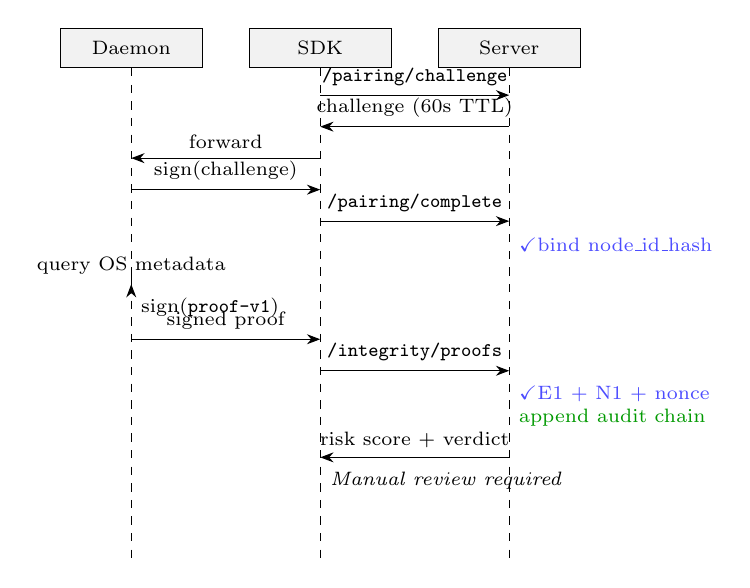
\begin{tikzpicture}[
  >=Stealth,
  node distance=0.8cm,
  every node/.style={font=\scriptsize},
  box/.style={draw, fill=gray!10, minimum width=1.8cm, minimum height=0.5cm, align=center},
]
% Actors
\node[box] (daemon) at (0,0)   {Daemon};
\node[box] (sdk)    at (2.4,0) {SDK};
\node[box] (srv)    at (4.8,0) {Server};

% Lifelines
\draw[dashed] (daemon.south) -- (0,-6.5);
\draw[dashed] (sdk.south)    -- (2.4,-6.5);
\draw[dashed] (srv.south)    -- (4.8,-6.5);

% 1. Pairing challenge
\draw[->] (2.4,-0.6) -- node[above]{\texttt{/pairing/challenge}} (4.8,-0.6);
\draw[->] (4.8,-1.0) -- node[above]{challenge (60s TTL)} (2.4,-1.0);
\draw[->] (2.4,-1.4) -- node[above]{forward} (0,-1.4);

% 2. Sign challenge
\draw[->] (0,-1.8) -- node[above]{sign(challenge)} (2.4,-1.8);
\draw[->] (2.4,-2.2) -- node[above]{\texttt{/pairing/complete}} (4.8,-2.2);
\node[right, color=blue!70] at (4.8,-2.5) {\checkmark bind node\_id\_hash};

% 3. Proof cycle
\draw[->] (0,-3.0) -- node[above]{query OS metadata} (0,-3.0);
\node[right] at (0,-3.3) {sign(\texttt{proof-v1})};
\draw[->] (0,-3.7) -- node[above]{signed proof} (2.4,-3.7);
\draw[->] (2.4,-4.1) -- node[above]{\texttt{/integrity/proofs}} (4.8,-4.1);
\node[right, color=blue!70] at (4.8,-4.4) {\checkmark E1 + N1 + nonce};
\node[right, color=green!60!black] at (4.8,-4.7) {append audit chain};

% 4. Risk
\draw[->] (4.8,-5.2) -- node[above]{risk score + verdict} (2.4,-5.2);
\node[right] at (2.4,-5.5) {\textit{Manual review required}};

\end{tikzpicture}
\caption{Simurgh proof protocol. Pairing binds the session to one node. Each proof uses E1 (\texttt{node\_id\_hash} $\wedge$ pubkey $\wedge$ signature) and N1 (paired-node continuity). All results append to the HMAC audit chain.}
\label{fig:protocol}
\end{figure}

%% ===================================================================
%% SECTION VI: PLATFORM IMPLEMENTATIONS
%% ===================================================================
\section{Platform Implementations}

\subsection{macOS Device Shield}

The macOS daemon is implemented in Swift using the CryptoKit framework. It generates and stores an ECDSA P-256 signing key (\texttt{P256.Signing.PrivateKey}) in the macOS Keychain at first launch under the account \texttt{p256-signing-key}. The daemon exposes a \texttt{127.0.0.1}-bound HTTP listener for proof and pairing endpoints. The OS scanner queries \texttt{CGWindowListCopyWindowInfo} with the combined \texttt{kCGWindowListOptionOnScreenOnly~|~kCGWindowListExcludeDesktopElements} mask and reads the \texttt{kCGWindowSharingState} property for each returned window. Its \texttt{signals} sub-object reports \texttt{node\_uptime\_ms}, \texttt{window\_count}, \texttt{capture\_excluded\_window\_count} (windows with sharing state \texttt{kCGWindowSharingNone}), and \texttt{helper\_status}. ScreenCaptureKit~\cite{apple2025screencapturekit} availability is exposed to the verifier as the \texttt{screencapturekit\_available} capability flag for forward compatibility; the current scanner remains single-path CoreGraphics, and an adaptive ScreenCaptureKit query path is reserved as a future-stage upgrade while preserving the metadata-only contract.

\subsection{Windows Device Shield}

The Windows daemon is implemented in .NET, using \texttt{ECDsa.Create(ECCurve.NamedCurves.nistP256)} for proof signing. The Windows scanner enumerates all top-level windows using \texttt{EnumWindows} and calls \texttt{GetWindowDisplayAffinity} on each handle. It counts windows with \texttt{WDA\_MONITOR} and \texttt{WDA\_EXCLUDEFROMCAPTURE} flags and reports them in the signed proof as \texttt{capture\_excluded\_window\_count} (umbrella: \texttt{capture\_restricted\_window\_count}) and \texttt{monitor\_only\_window\_count}. No window title, class name, process name, or PID is included in the summary; the raw window handle is used only transiently during enumeration and is never written to the proof. Real-device validation on Windows~10 Pro build~19045 confirmed correct detection of both flags, signed proof submission, server-side acceptance, and correct propagation of the affinity count into the risk score, dashboard, and audit chain.

\subsection{Linux Display Integrity Research}

The Linux daemon is implemented in Rust, using the \texttt{p256::ecdsa} crate for proof signing. Due to the diversity of the Linux desktop landscape, the Linux implementation is positioned as a display integrity research contribution rather than a complete deployment target. Three scanner paths are implemented:

\textbf{X11}: The Rust daemon connects to the X server via \texttt{x11rb} and enumerates top-level windows. It reads the \texttt{\_NET\_WM\_STATE} property and window manager hints to identify windows exhibiting overlay-relevant window-manager states. \texttt{capture\_excluded\_window\_count} is reported. No window title or class is read.

\textbf{Wayland}: Direct window enumeration is not available to unprivileged clients in Wayland. The daemon probes the \texttt{org.freedesktop.portal.Desktop} service via D-Bus using \texttt{NameHasOwner} (to detect portal presence) and reads the \texttt{ScreenCast.AvailableSourceTypes} property (to detect active screencast capability). It never calls \texttt{CreateSession}, \texttt{SelectSources}, \texttt{Start}, or \texttt{OpenPipeWireRemote}~--- the portal methods that would trigger a user consent prompt. A banned-method grep test in CI enforces this invariant.

\textbf{XWayland}: The X11 scanner path runs against the \texttt{\$DISPLAY} provided by XWayland, providing partial coverage of applications running in XWayland compatibility mode. Coverage is reported as \texttt{coverage=xwayland\_partial} in the proof.

A display-server lock prevents proof acceptance from sessions where the detected display server does not match the expected type, providing defence against display-server spoofing.

\subsection{Cross-Platform Verification Contract}

The macOS, Windows, and Linux daemons do not emit byte-identical envelopes across all implementation stages. Instead, they satisfy a shared verification contract: each proof is session-bound, challenge-bound, timestamped, signed by a registered node key, privacy-normalised, and processed by the server through the same signature check (E1), replay guard, node-continuity rule (N1), raw-field rejection, risk mapping, and audit-chain append pipeline. The canonical serialisation (\texttt{proofCanonicalise.js}) is mirrored in Swift (\texttt{ProofSigner.swift}) and Rust (\texttt{canonical\_json.rs}), with byte-identical golden fixture tests enforcing cross-implementation consistency for the fields shared between envelope types.

%% ───────────────────────────────────────────────────────────────────
%%  Table III: Platform Capability Matrix
%% ───────────────────────────────────────────────────────────────────
\begin{table}[t]
\centering
\small
\caption{Platform Capability Matrix}
\label{tab:platform}
\resizebox{\columnwidth}{!}{%
\begin{tabular}{@{}lllll@{}}
\toprule
\textbf{Platform} & \textbf{Signal source} & \textbf{Impl.} & \textbf{Validation} & \textbf{Known limitation} \\
\midrule
macOS & \texttt{kCGWindowSharingState} & Swift/CoreGraphics & Swift tests (8) & SCKit adaptive path deferred \\
Windows & \texttt{WDA\_MONITOR}, \texttt{WDA\_EXCLUDEFROMCAPTURE} & .NET/Win32 & Real device (Win10 19045) & No kernel/GPU overlay visibility \\
Linux X11 & Window-manager states (\texttt{\_NET\_WM\_STATE}) & Rust/x11rb & CI + Xvfb & Real desktop pending \\
Linux Wayland & Portal metadata only & Rust/D-Bus & Mock D-Bus + CI & No surface enumeration \\
XWayland & X11 bridge (partial) & Rust/x11rb & CI & Partial coverage only \\
\bottomrule
\end{tabular}%
}
\end{table}

%% ===================================================================
%% SECTION VII: PRIVACY MODEL
%% ===================================================================
\section{Privacy Model}

\subsection{Metadata-Only Collection}

Simurgh's privacy model distinguishes between \textit{behavioural metadata} (what the student did) and \textit{content} (what the student wrote, said, or displayed). Only the former is collected; Table~\ref{tab:privacy} specifies the boundary for each signal class.

\begin{table}[t]
\centering
\small
\caption{Privacy Collection Boundary}
\label{tab:privacy}
\resizebox{\columnwidth}{!}{%
\begin{tabular}{@{}lll@{}}
\toprule
\textbf{Signal} & \textbf{Collected} & \textbf{Never collected} \\
\midrule
Keystrokes & Count per window & Keystroke content \\
Characters typed & Count only & Typed text \\
Paste events & Count + char length & Paste content \\
Focus loss & Count + duration (ms) & Window title/target \\
Idle gaps & Maximum gap (ms) & Content during idle \\
WPM & Effective WPM & Text being typed \\
Timing intervals & Up to 200 samples & Key content \\
Display affinity & Window count & Titles, PIDs, names \\
Student identity & SHA-256 hash & Raw identifier \\
\bottomrule
\end{tabular}%
}
\end{table}

\subsection{Forbidden Fields}

The following data types are explicitly forbidden at every layer of the system: screen pixels; webcam frames; microphone audio; typed content; pasted content; raw window titles; raw window class names; raw process names; process identifiers; window handles; raw public keys in audit payloads (only hashes are stored); hardware serial numbers; MAC addresses; hostnames; and personal device identifiers. The \texttt{node\_id\_hash} field is a pseudonymous verifier identifier derived from the daemon public key; it is used only for session and node continuity and does not expose any hardware or user identity. The proof schema validator and privacy audit scripts enforce these constraints as regression gates.

\subsection{No Screen, Audio, Webcam, or Content Collection}

Simurgh does not implement and does not call \texttt{getDisplayMedia()}, \texttt{getUserMedia()} with video or audio, any screenshot API, any audio capture API, or any clipboard-read API. The browser SDK does not attach any event listener that could capture content. These non-implementations are verified in the privacy audit that runs as part of the CI check suite.

\subsection{Manual Review Only}

Critical verdicts are accompanied by the hard-coded string ``Manual review required. No automatic misconduct finding.'' Warning verdicts produce ``Manual review recommended. No automatic misconduct finding.'' Neither string can be suppressed through configuration. The system produces no binary misconduct verdict, no suspension action, no notification to any authority, and no persistent record outside the instructor-accessible audit export. All conclusions require a human reviewer.

%% ===================================================================
%% SECTION VIII: EVALUATION
%% ===================================================================
\section{Evaluation}

\subsection{Functional Validation}

Table~\ref{tab:eval} summarises the automated validation results across the prototype.

\begin{table}[t]
\centering
\small
\caption{Automated Validation Summary}
\label{tab:eval}
\resizebox{\columnwidth}{!}{%
\begin{tabular}{@{}lll@{}}
\toprule
\textbf{Suite} & \textbf{Runtime} & \textbf{Result} \\
\midrule
Node.js unit tests & Node.js 22 & 327 / 327 pass \\
Rust daemon tests & Rust stable & 33 / 33 pass \\
Windows .NET tests & .NET 8 & 11 / 11 pass \\
macOS Swift daemon tests & Swift/Xcode & 8 / 8 pass \\
Stage 2.7 cross-platform smoke & Node.js + Rust & All scenarios pass \\
Stage 2.8 Linux smoke & Node.js + Rust & 16 scenarios pass \\
Security audit assertions & Node.js & 30 / 30 pass \\
Privacy audit gates & Node.js & All pass \\
npm advisory audit & npm & 0 high/critical \\
\bottomrule
\end{tabular}%
}
\end{table}

The Node.js unit tests cover the proof validator, pairing registry, nonce guard, HMAC chain, risk scorer, session state machine, telemetry normaliser, and report builder. Rust tests cover the Linux daemon scanner paths (X11, Wayland, XWayland), the cross-platform canonicalisation implementation, and the Linux daemon proof flow; macOS daemon correctness is covered by the Swift test suite (\texttt{AffinityScannerTests.swift}, \texttt{ScannerProofTests.swift}, \texttt{PrivacyNormaliserTests.swift}, \texttt{DaemonDoctorTests.swift}; 8 tests). The Windows .NET tests exercise the display-affinity scanner and signed proof contract.

\subsection{Security Audit}

A ten-question internal security audit evaluated the proof protocol against the following threat scenarios: pairing replay, browser-forged \texttt{signature\_status}, macOS key protection, challenge single-use and expiry, node continuity per session, audit hint spoofing, rate-limit sizing, browser trust boundary, audit emission on rejection, and demo failure state reproducibility. All ten questions received positive answers with code-level evidence and regression gate coverage~(10/10).

An additional 30-assertion cybersecurity audit across 16 security dimensions was conducted for the Stage~2.8 Linux path, covering: nonce handling, signature verification, replay protection, display-server lock, Wayland consent safety, XWayland partial coverage boundary, audit completeness, rate limiting, privacy contract, anti-overclaiming wording, and CI enforcement. All 30 assertions pass.

\subsection{Privacy Audit}

The privacy audit verifies the following properties as regression-gated checks: (1)~no \texttt{window.getDisplayMedia()} call in the browser SDK or server; (2)~no clipboard-read API call; (3)~no \texttt{getUserMedia()} call with video or audio; (4)~no raw window title or process name in any proof schema field; (5)~no raw student identifier written past the ingress hasher; (6)~no raw private key or raw public key in any audit chain entry; (7)~forbidden Wayland portal methods absent from the Rust scanner. These checks run as part of the \texttt{scripts/check.sh} gate suite on every CI run.

\subsection{Real-Device Windows Validation}

The Windows Device Shield was validated on a physical Windows~10 Pro machine (build~19045). The validation confirmed: \texttt{WDA\_MONITOR}-flagged windows increment \texttt{monitor\_only\_window\_count} (and the umbrella \texttt{capture\_restricted\_window\_count}); \texttt{WDA\_EXCLUDEFROMCAPTURE}-flagged windows increment \texttt{capture\_excluded\_window\_count}; unflagged windows contribute to neither counter. Signed proofs from the .NET daemon were accepted by the Node.js verifier; tampered proofs, replayed nonces, and wrong-node proofs were rejected with correct reason codes and audit entries. The affinity counts propagated correctly into the risk score, the instructor report, and the audit chain export.

\subsection{Linux CI and Display-Server Validation}

Ubuntu CI validation runs the full Linux Rust test suite under mandatory \texttt{Xvfb} with \texttt{SIMURGH\_REQUIRE\_XVFB\_TESTS=1}. Shellcheck linting enforces all lifecycle scripts. The Wayland probe path is validated via a mock D-Bus environment. Display-server mismatch enforcement is tested via the 16-scenario smoke suite, which includes headless, X11, XWayland, and Wayland-advertised configurations. The CI pipeline rejects any run where Xvfb is missing when the flag is set, preventing false-pass results on headless runners.

\subsection{LLM-Assisted Development Methodology}

The proof protocol, risk scorer, platform daemon implementations, test suites, and audit gate framework were developed using Claude Code powered by Anthropic's Claude Sonnet~4.6. The LLM was used as an implementation assistant under explicit anti-overclaiming constraints derived from the RESEARCH\_PROGRAMME.md document. All non-claims were manually verified. This disclosure follows the methodology transparency standard established in~\cite{abedini2026invisible}.

%% ===================================================================
%% SECTION IX: SECURITY ANALYSIS
%% ===================================================================
\section{Security Analysis}

\subsection{What Simurgh Detects}

Simurgh produces integrity signals for the following anomalies at the metadata level:
\begin{itemize}
\item Presence of capture-excluded windows (\texttt{WDA\_EXCLUDEFROMCAPTURE}, \texttt{WDA\_MONITOR}, \texttt{SharingType.none}) during an active session.
\item Abnormal paste behaviour (high paste count, large paste character volumes).
\item Unusual focus-loss patterns (high loss count, long accumulated duration).
\item Anomalous typing patterns (WPM far outside baseline, irregular keydown timing distribution).
\item Extended idle periods inconsistent with active exam behaviour.
\item Daemon proof failure events (replay, signature failure, node mismatch) indicating potential daemon tampering.
\item Session-level anomalies (premature disconnect, irregular state transitions).
\end{itemize}

\subsection{What Simurgh Cannot Detect}

The following attack classes are explicitly outside the current system boundary:

\textbf{GPU-layer overlays}: Tools that hook DirectX or Metal compositor layers and render directly to the GPU display output bypass both the OS window-management APIs and any capture pipeline. No OS-level window enumeration will see these overlays. This limitation is documented in the Stage~1 limitations document and the RESEARCH\_PROGRAMME.md.

\textbf{Read-only workflows}: A student who silently reads from a second device, printed notes, or a physical reference without interacting with a capture-invisible overlay will produce no anomalous signals in the Simurgh data stream. Gaze-tracking approaches exist~\cite{kaddoura2023computational,ferdosi2023modeling} but are explicitly out of scope for this system.

\textbf{Kernel-level compromise}: A compromised operating system or kernel-level rootkit can modify the return values of any API the daemon queries. No user-space tool can detect this. Hardware-rooted attestation (Section~XII-B) is the long-term direction.

\textbf{Click-through overlays without display-affinity flag}: A click-through overlay that does not set a capture-exclusion flag is not detectable through the affinity scanner. Browser focus-loss events may trigger if the user clicks, but a purely read-only click-through overlay with no keyboard interaction may produce no signal.

\subsection{Tamper and Replay Resistance}

The HMAC-SHA256 audit chain makes retroactive modification of any event record detectable by any verifier holding the HMAC key. The nonce guard prevents replaying a valid proof from one session epoch into another. The E1 triple check (hash + key + signature) prevents forging a proof that appears to come from a registered node. The N1 node-continuity invariant prevents an adversary from switching daemons mid-session after an initial pairing. Rate limits (30 proof submissions per minute, 10 pairing challenges per minute) bound amplification attacks.

\subsection{Remaining Attack Surface}

An adversary who can run the Simurgh daemon client unmodified but controls the proof's \texttt{signals} sub-object (or, in the daemon envelope, the affinity-count fields) through OS-level manipulation can submit a dishonest but validly signed proof. The server cannot distinguish a lying daemon from an honest one if the signing key is genuine and the proof format is correct. Signed proofs attest identity (\textit{this key submitted this data}) but not truthfulness (\textit{this data faithfully reflects OS state}). Hardware-rooted attestation, discussed in Section~XII-B, addresses this gap. Until then, the proof architecture provides meaningful replay and forgery resistance while being honest about the remaining trust assumption.

%% ===================================================================
%% SECTION X: ETHICS AND DEPLOYMENT LIMITS
%% ===================================================================
\section{Ethics and Deployment Limits}

\subsection{No Automatic Misconduct Finding}

Simurgh is designed explicitly as an evidence-gathering tool for human reviewers, not a disciplinary decision engine. The hard-coded ``Manual review required'' wording in the risk scorer is not a UI choice; it reflects an architectural commitment. The system does not produce a verdict, flag a student to any authority, or trigger any automated action. A high risk score is a recommendation for a human to look at the session's audit chain, not a finding of misconduct.

\subsection{Research Prototype Status}

Project Simurgh is a research prototype at version~0.4.18. It has not been reviewed by any data-protection authority, accessibility auditor, or institutional ethics board beyond the development team's own review process. It has not been piloted with actual students in any live examination context. Institutional deployment would require, at minimum: a formal data-protection impact assessment (FERPA, GDPR, or equivalent); an accessibility review against WCAG~2.2~AA; an external red-team engagement; signed and notarised macOS/Windows distribution packages; and an institutional pilot under ethics oversight.

The system should not be described as production-ready, compliant with any specific framework without naming the assessment, or ready for deployment by universities without the above-listed review processes.

\subsection{Institutional Review Requirements}

The staged deployment roadmap in the Simurgh RESEARCH\_PROGRAMME identifies the following gates before any regulated-environment use: privacy/legal review (including data retention and student-access policies), accessibility review, external red-team engagement (pairing replay, helper spoofing, audit chain manipulation), signed distribution pipeline, and LMS integration design. None of these gates are currently passed. We include this explicit statement in accordance with the ACM and IEEE codes of ethics~\cite{acm2018code,ieee2024code}.

%% ===================================================================
%% SECTION XI: RELATED WORK
%% ===================================================================
\section{Related Work}

\subsection{Proctoring System Security and Criticism}

Simko et al.~\cite{simko2024modern} catalogue community-developed proctoring evasion techniques, documenting the adversarial dynamic between proctoring systems and test-takers. Their taxonomy includes the display-affinity subclass that Simurgh directly addresses. Balash et al.~\cite{balash2023educators,balash2021examining} examine educator and student perspectives, documenting the privacy and usability costs of existing systems. Luijben et al.~\cite{luijben2024security} formalise five security requirements; Simurgh addresses Requirement~2 (work authenticity) through the proof architecture while preserving Requirement~4 (data protection) through the metadata-only model.

\subsection{Behavioural Detection}

A substantial body of work applies gaze tracking~\cite{kaddoura2023computational,ferdosi2023modeling}, mouse dynamics~\cite{wang2020user}, keystroke analysis, and multimodal fusion~\cite{guan2021design,atoum2017automated} to exam integrity. Simurgh collects behavioural signals in the same spirit but differs in two important ways: (1) it collects count-level metadata rather than biometric streams; and (2) it pairs behavioural signals with cryptographic device proofs rather than treating browser-observable signals as the sole evidence source.

\subsection{Hardware Attestation and Zero Trust}

The NIST Zero Trust Architecture~\cite{nist2020zerotrust} framework motivates treating the client device as untrusted until it provides verifiable proof of identity and state. Simurgh's signed proof envelope (Ed25519 for the browser-paired proof path, ECDSA P-256 for the device-shield daemons) is a software instantiation of this principle, pending hardware-rooted attestation. Trusted Platform Module~\cite{tpm2spec} and Intel TXT provide hardware-backed attestation primitives; WebAuthn~\cite{w3c2021webauthn} provides a browser-accessible version using platform authenticators. Simurgh's architecture is designed to accept hardware-rooted proofs in a future stage (Section~XII-B) without breaking the existing proof contract.

\subsection{Privacy-First Assessment}

Paris et al.~\cite{paris2021sins} and Mukherjee et al.~\cite{mukherjee2024balancing} document the privacy limitations of current proctoring systems. Duncan and Joyner~\cite{duncan2022necessity} argue for alternative assessment designs that are structurally resistant to cheating. Prinsloo et al.~\cite{prinsloo2024vulnerable} identify AI-powered educational decision systems as a vulnerability for student well-being. Simurgh's metadata-only model is a direct response to these concerns: by design, it cannot produce the surveillance record that existing systems create.

%% ===================================================================
%% SECTION XII: DISCUSSION AND FUTURE WORK
%% ===================================================================
\section{Discussion and Future Work}

\subsection{Agent Shield}

Stage~3 of the Simurgh roadmap introduces an Agent Shield: a proof-based integrity layer for AI computer-use sessions, where an LLM agent performs tasks on behalf of the session holder. Agent-mediated sessions present a distinct integrity surface, as the agent itself is a new attack vector (tool poisoning, prompt injection, system-prompt leakage). The Agent Shield will extend the existing proof envelope to include an agent attestation field: a signed summary of the agent's visible tool invocations and reasoning traces, bounded by the same metadata-only privacy contract.

\subsection{Hardware-Rooted Attestation}

The current Ed25519 + ECDSA P-256 proof architecture provides software-level identity binding: the proof attests that \textit{this key signed this data at this time}. It does not attest that the data faithfully reflects the OS state, because the key itself resides in user space. Hardware-rooted attestation via TPM~\cite{tpm2spec} or Secure Enclave would move the signing key into hardware, making it non-extractable and binding the attestation to physical device identity. Apple's Secure Enclave and Windows' TPM~2.0 both provide the necessary primitives; the challenge is integrating them into the existing proof contract without breaking the metadata-only privacy model. Attestation keys must not leak device identity across sessions.

\subsection{Privacy-Preserving Visual Verification}

Stage~4 explores the possibility of recovering some visual integrity signal without collecting screen pixels. Approaches under consideration include on-device inference of scene-level properties (``student is seated at a desk'') using a private enclave, rather than cloud video analysis; homomorphic comparisons of frame hashes without transmitting content; and hardware display-output attestation using HDCP link integrity signals. All of these approaches face significant engineering challenges and are research directions rather than near-term plans.

%% ===================================================================
%% SECTION XIII: CONCLUSION
%% ===================================================================
\section{Conclusion}

This paper has presented Project Simurgh, a privacy-preserving integrity architecture for high-stakes AI-mediated and remote assessment sessions. We have shown that the display-fidelity failure documented in the Invisible Window attack~\cite{abedini2026invisible} — the gap between the physical display and the screen-capture surface — can be addressed without resorting to more invasive surveillance. Instead, Simurgh establishes session integrity through signed, metadata-only device proofs, native OS display-affinity scanners, and a tamper-evident audit chain.

The core architectural argument is straightforward: if the OS compositing pipeline cannot be trusted to faithfully expose all visible content to the browser capture API, then the appropriate response is to move the trust anchor to the OS level itself, where the capture-exclusion state is visible to any native process. Simurgh does exactly this, at the price of requiring a native daemon on the student's device — a cost that is explicit and reasonable, compared to the alternative of collecting full screen video.

The four contributions of this work — the privacy-preserving architecture, the cross-platform prototype, the display-affinity detection without content capture, and the evaluated manual-review-only decision model — represent a concrete existence proof that capture-resistant integrity assessment is technically feasible while preserving meaningful privacy guarantees. We hope this work encourages further research into proof-based, metadata-only integrity systems and provides a documented, auditable foundation for institutional engagement.

\section*{Acknowledgements}

This research was conducted using Claude Code powered by Anthropic's Claude Sonnet~4.6. The author thanks Anthropic for providing the research tooling. This paper is a companion to the Invisible Window disclosure paper~\cite{abedini2026invisible}, which documented the motivating attack class. The author thanks the reviewers of the Simurgh RESEARCH\_PROGRAMME and Stage~2 closeout documentation for their feedback on the non-claims posture adopted throughout this work.

{\sloppy
\bibliographystyle{IEEEtran}
\bibliography{references}
}

\end{document}
